%\section{Getting Canopy Python}
%
%If you choose the Canopy system, follow these instructions. You may already
%have the Canopy distribution of Python. If so skip down to adding PySerial
%in the next section.
%
%Canopy is a little more polished in it's setup. And it works well. So let's
%see how to install this version of Python and enhance it with the Pyserial
%library. We will start at the Canopy home site
%https://www.enthought.com/products/canopy/. Partway down the page there is a
%blue \textquotedblleft Download Canopy\textquotedblright\ button.
%
%\begin{figure}[h!]
%
\includegraphics[width=3.0219in,height=1.7988in]{PH4CAU2C}
%\end{figure}This will take you to the
%download page where you can choose the version for your operating system.
%When you click the proper download link, it will ask you for some
%information. \begin{figure}[h!]
	%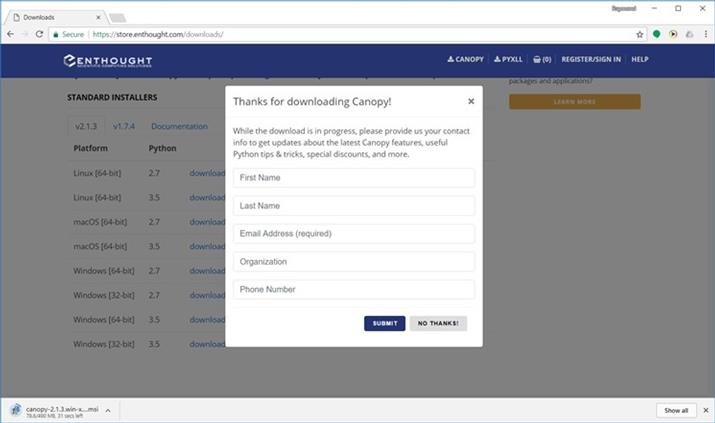
\includegraphics[width=6.0164in,height=3.5674in]{PH4CAU2D}
	%\end{figure}
	%
	%Once the download completes, install Canopy. When you run the program, you
	%will see something like this\begin{figure}[h!]
		%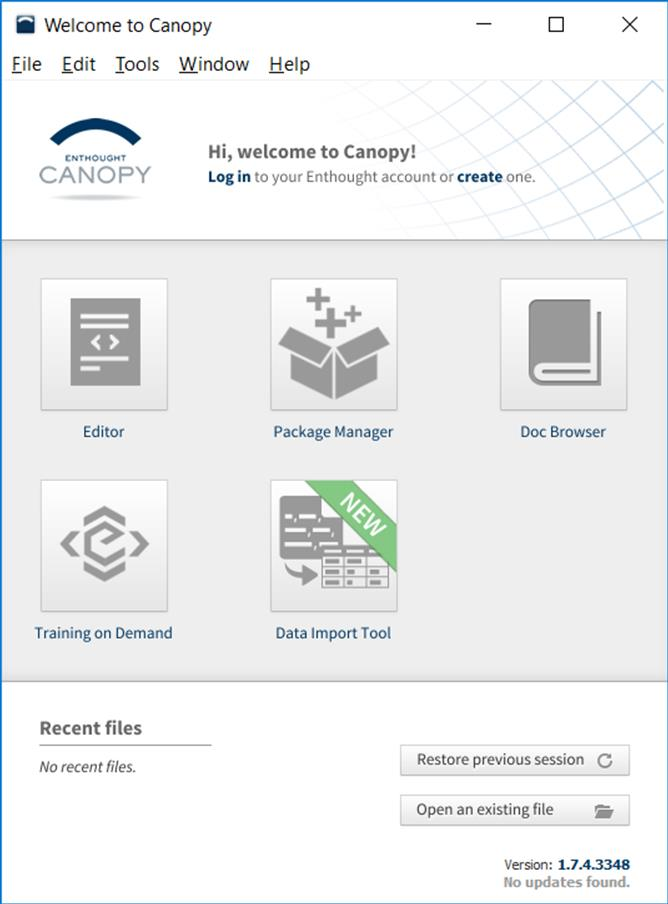
\includegraphics[width=1.983in,height=2.6775in]{PH4CAU2E}
		%\end{figure}
		%
		%The editor lets us write Python programs. If you choose this you get a
		%window like our Arduino program. \begin{figure}[h!]
			%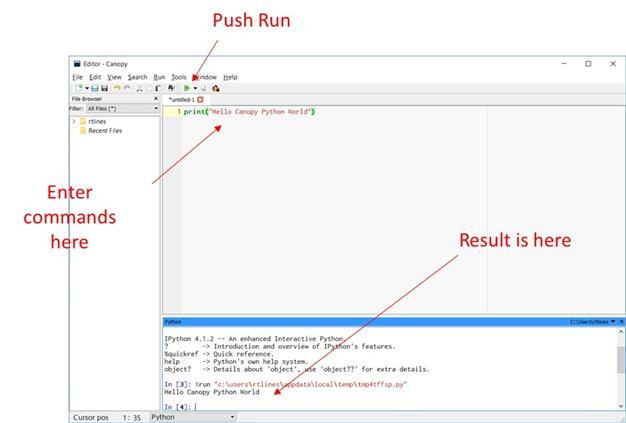
\includegraphics[width=5.2641in,height=3.563in]{PH4CAU2F}
			%\end{figure}The editor is a place to write
			%and run Python commands very like our Arduino softare. Only, this time there
			%is no checking and uploading the code, because the Python code will run on
			%our computer, not on an Arduino.
			%
			%In the figure above, the command just says to print \textquotedblleft Hello
			%Canopy Python World\textquotedblright\ and that is all. When it runs, it
			%prints our message on the small window at the bottom of the Editor window.
			%But of course Python can do much more than print silly messages in little
			%windows. We will have our Python system read a serial port and save our data
			%to a file. But we need an additional piece of Python to do this. We need
			%functions that can handle serial ports. These functions are already written
			%by someone, and put together in a package called a \textquotedblleft
			%library.\textquotedblright\ But this library isn't included in what we have
			%downloaded, so we need to fix this next.
			%
			%\subsection{Getting the PySerial library for Canopy\label{Canopy}}
			%
			%Now that we have Python, we need to update it with the PySerial library so
			%that we can read our data from the computer serial port. If we go back to
			%the Canopy main window we will see a \textquotedblleft Package
			%Manager.\textquotedblright\ The Package manager lets us add new parts of
			%Python, and that is just what we want to do. Choose the Package Manager and
			%in its search box type in \textquotedblleft pyserial.\textquotedblright 
			%\begin{figure}[h!]
			%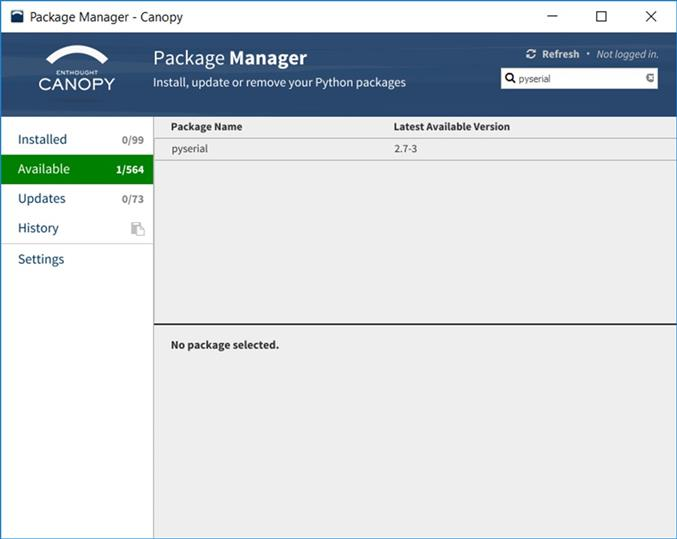
\includegraphics[width=3.9302in,height=3.1328in]{PH4CAU2G}
			%\end{figure}
			%
			%It won't initially find pyserial because it is not yet installed and we are,
			%by default, looking at what is installed. But choose the \textquotedblleft
			%Available\textquotedblright\ tab. Now we see pyserial in the package list.
			%Select Pyserial\begin{figure}[h!]
				%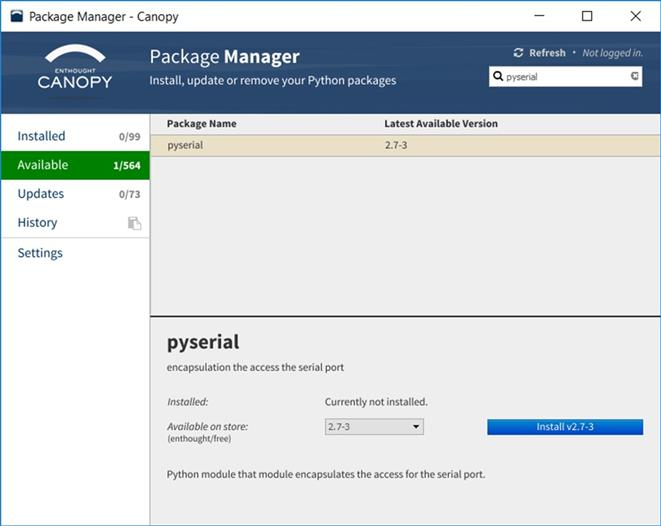
\includegraphics[width=4.0588in,height=3.233in]{PH4CAV2H}
				%\end{figure}and choose the install button
				%that appears. If all goes well, you will see a red \textquotedblleft
				%uninstall\textquotedblright\ button appear.\begin{figure}[h!]
					%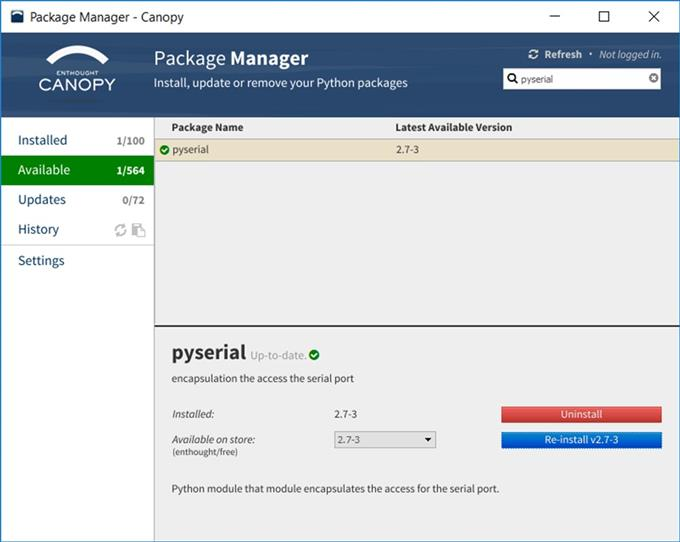
\includegraphics[width=4.4849in,height=3.5786in]{PH4CAV2I}
					%\end{figure}
					%
					%Now we can go back to the editor and write our code to read the serial port. 
					%\begin{figure}[h!]
					%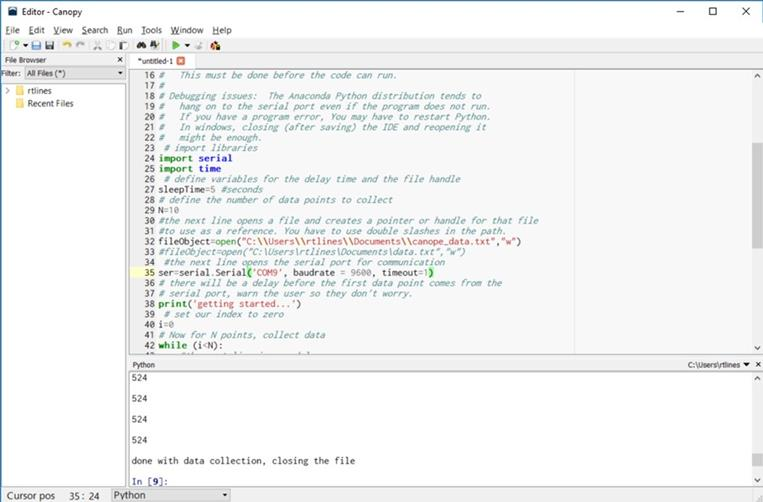
\includegraphics[width=5.227in,height=3.4442in]{PH4CAV2J}
					%\end{figure}